\subsection{Studies in the Uniform Phase Space} % (fold)
\label{sub:flat_hypercube_studies}

An important part of the investigation into what the neutral networks are learning beyond the standard physics features is to quantify the performance when these features are removed.  This represents the {\it unique information} learned by the network.  One way to remove the discrimination power from a given feature is to apply a transformation such that the marginal likelihood ratio is constant at unity.  In other words, we derive event-by-event weights such that

\begin{equation}
\label{eq:flat}
  f(m, \tau_{21}, p_T| W'\rightarrow WZ) \approx f(m, \tau_{21}, p_T| QCD),
\end{equation}

\noindent where $f(X|Y)$ is the probability density function of $X$ given $Y$.  This is done practically by binning the mass and $\tau_{21}$ distributions and then assigning to each event a weight given by the inverse bin content corresponding to the jet mass and $\tau_{21}$ of that particular event. Figure~\ref{fig:rocCube} shows the ROC curve for various features with this weighting scheme applied.  By construction, $\tau_{21}$ and the jet mass do not have any discrimination power between signal and background, evident by the fact that $\epsilon_\text{bkg} = \epsilon_\text{signal} = $ the random guess line.    However, the convolutional network that is trained inclusively (without the weights from Equation~\ref{eq:flat}) does have some discrimination power when the weights from Equation~\ref{eq:flat} are applied.  For a fixed signal efficiency, the overall performance is significantly degraded with respect to the un-weighted ROC curve in Figure~\ref{fig:combinedROC1}, but the improvement over a random guess is significant.  Interestingly, the network performance is significantly better in this re-weighted setting when the same weighting is applied during training (effort by the network is not needed to learn $\tau_{21}$, for instance).  The ConvNet and MaxOut procedures training inclusively have similar performance.

%$\epsilon_\text{bkg}(\epsilon_\text{signal})=\epsilon_\text{signal}$ (the random guess line)

One can gain intuition about the unique information learned by the network by studying the correlation of the network output and the pixel intensities with the Equation~\ref{eq:flat} weights applied.  This is shown in Figure~\ref{fig:cor_hyper} with and without the weights applied during training.  The two correlation plots are qualitatively similar, but the region to the right of the subjets is more enhanced when the weights are applied during the training.  This suggests that information about radiation surrounding the subjets contains important discrimination power contributing to the network's unique information.

\begin{figure}[htbp]
  \centering
 % 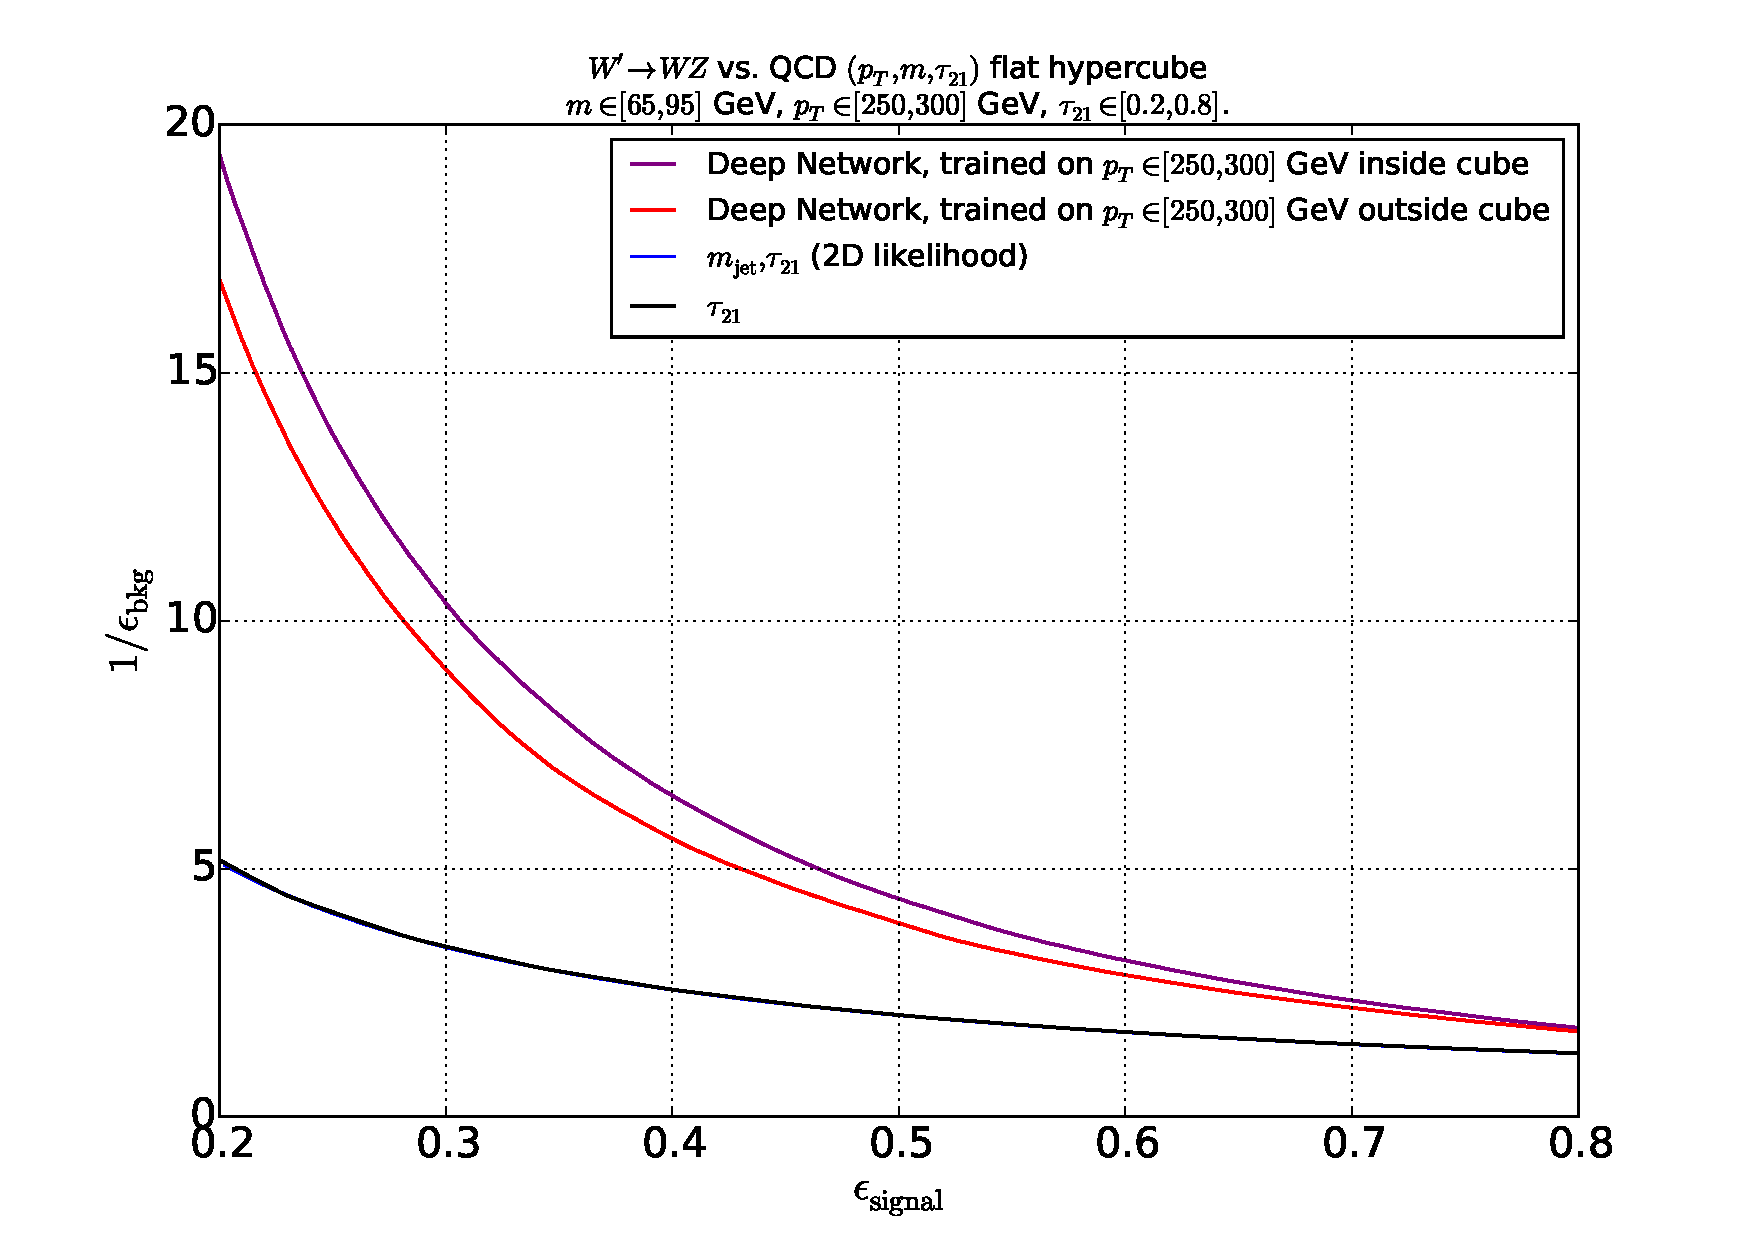
\includegraphics[width=0.95\textwidth]{figures/roc-cube-inside.pdf}
    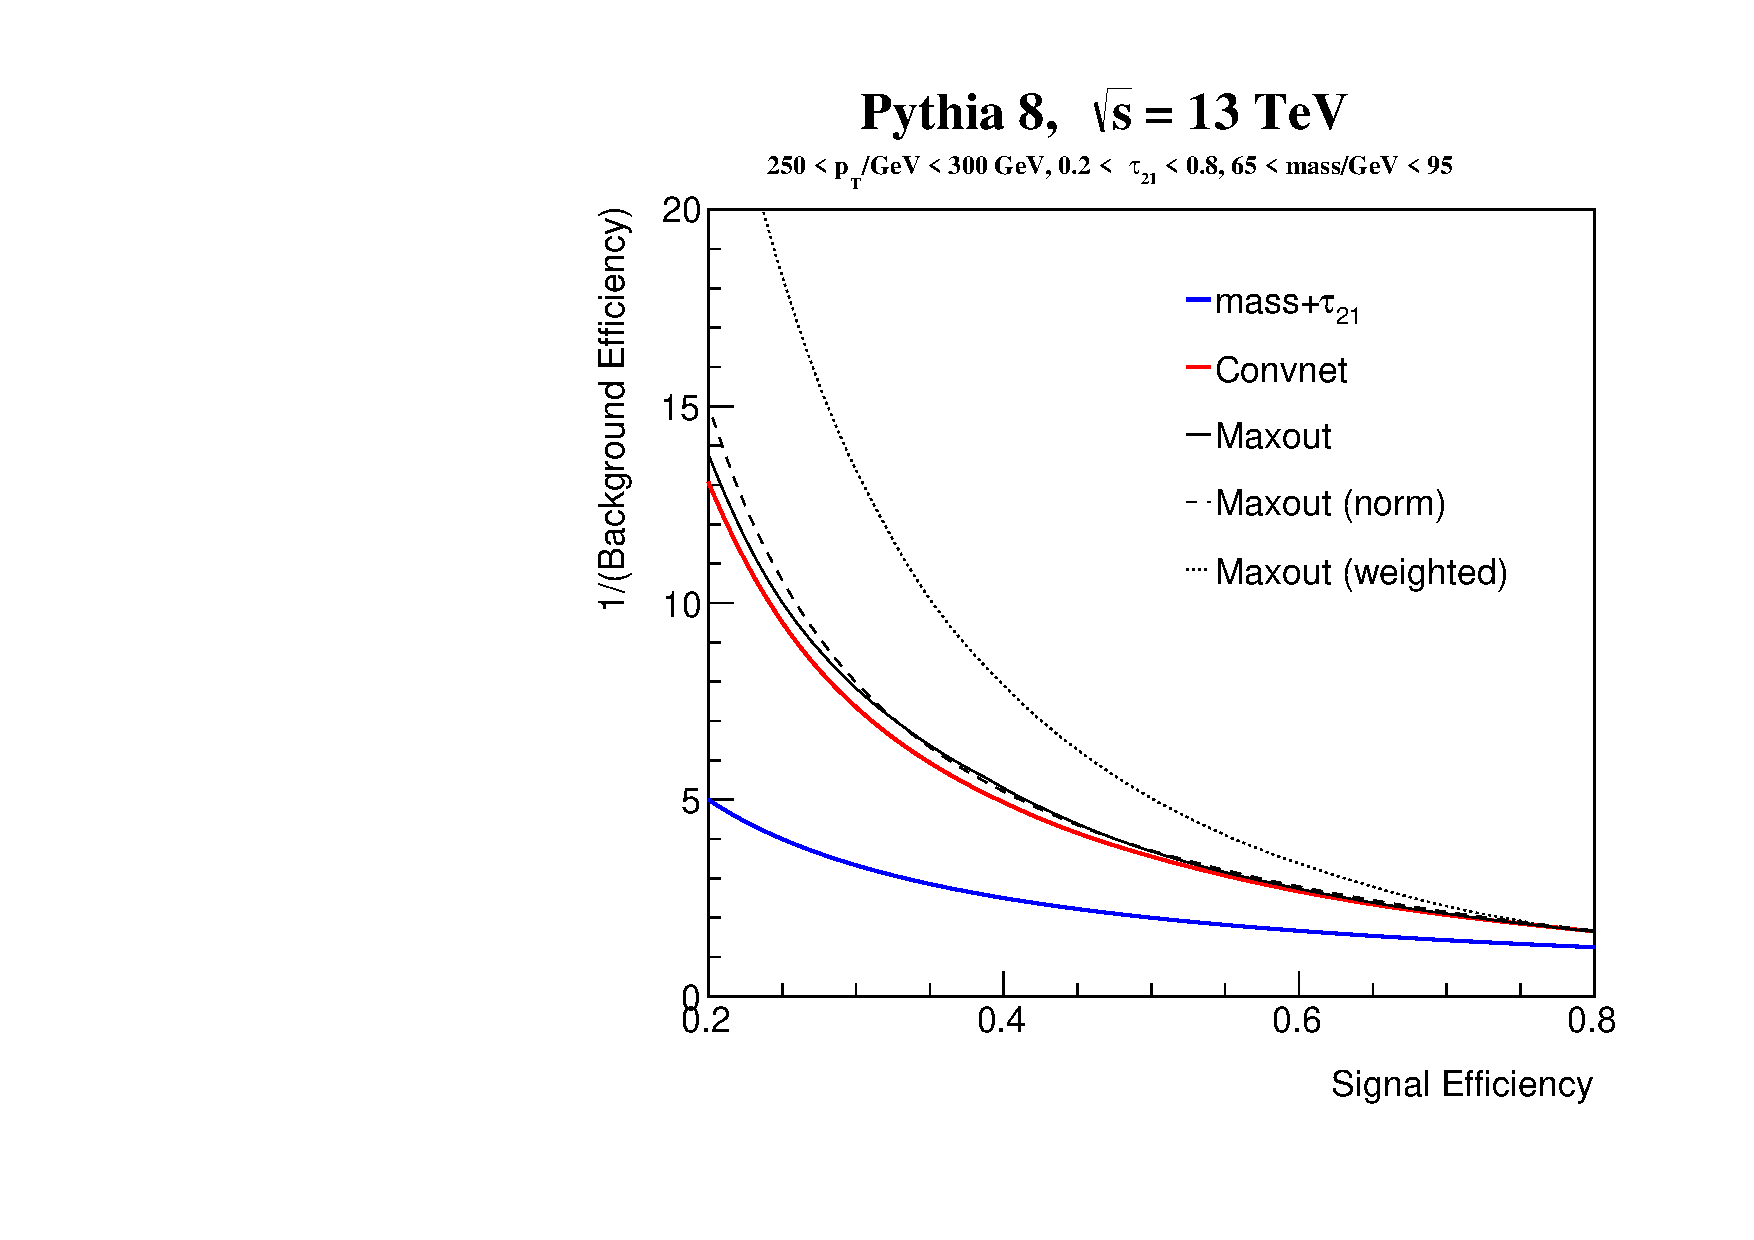
\includegraphics[width=0.5\textwidth]{figures/ROCs_window.pdf}
  \caption{Various ROC curves with event weights that enforce Eq.~\ref{eq:flat} inside $m\in[65, 95]$ GeV,  $p_T\in[250, 300]$ GeV, and  $\tau_{21}\in[0.2, 0.8]$.  By construction, the $\tau_{21}$ and likelihood combination of $\tau_{21}$ and mass are non-discriminating (and are thus equal to a random guess).  The ConvNet, MaxOut, and MaxOut-Norm networks are trained without the weights applied and the MaxOut (weighted) line was trained with the weights applied during training.}
  \label{fig:rocCube}
\end{figure}


\begin{figure}[htbp]
  \centering
  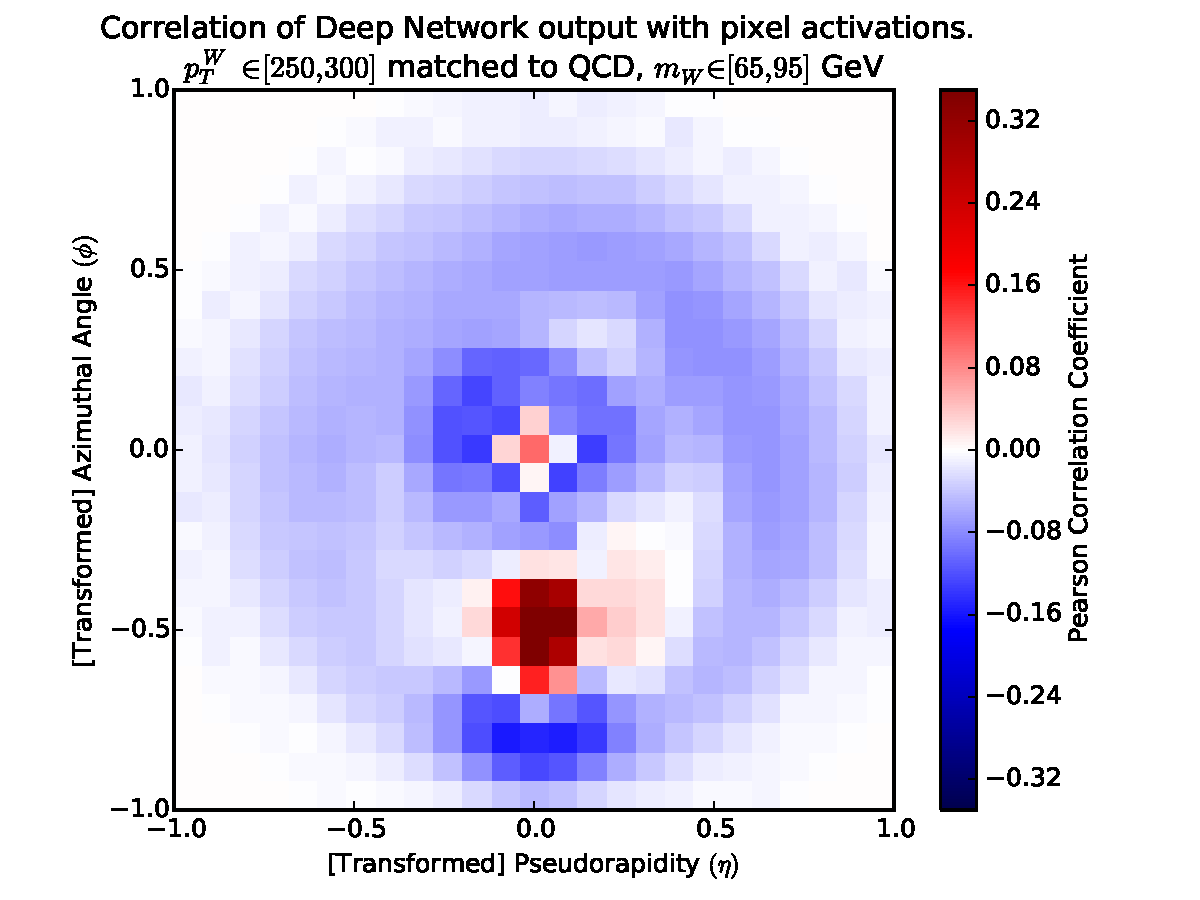
\includegraphics[width=0.45\textwidth]{figures/hypercube-pixel-activations-corr.pdf} 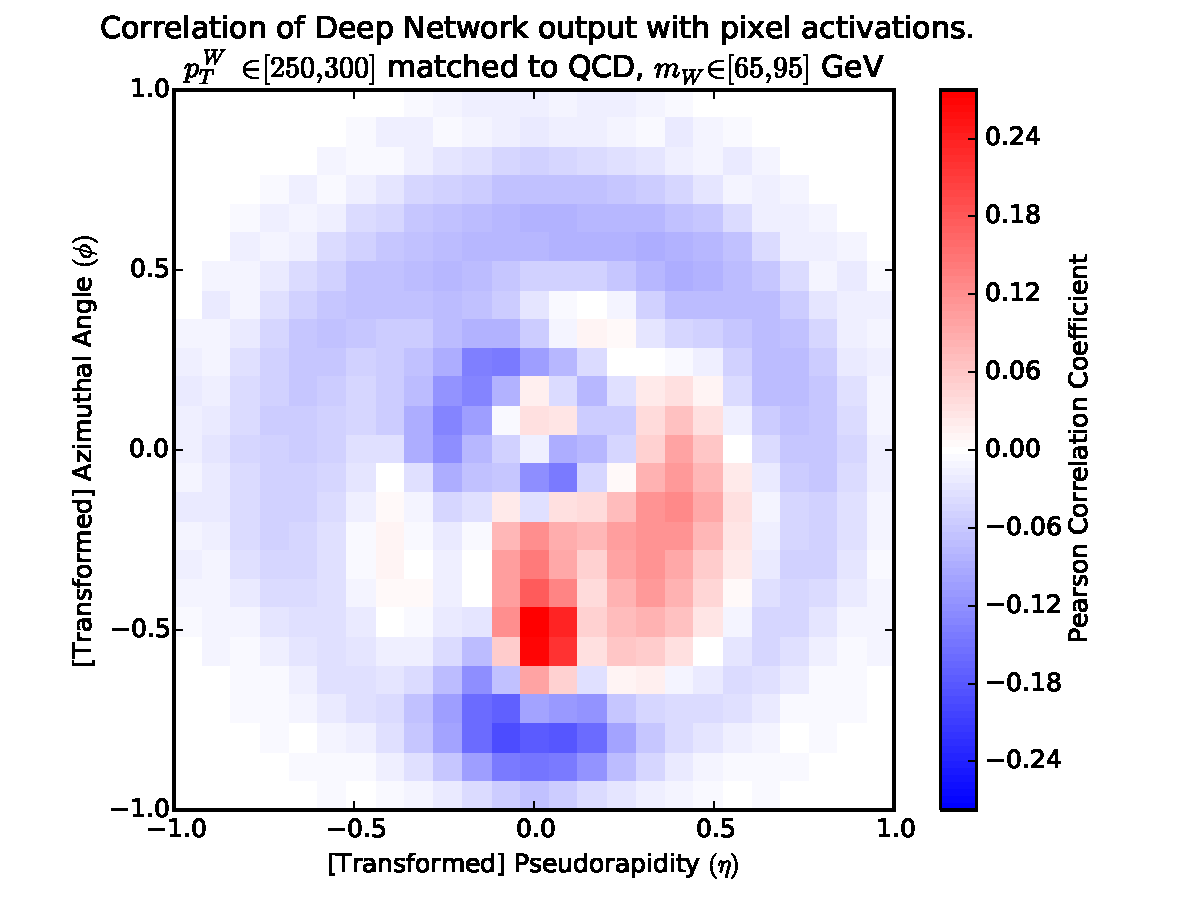
\includegraphics[width=0.45\textwidth]{figures/ahypercube-pixel-activations-corr.pdf}
  \caption{Pearson Correlation Coefficient for pixel intensity and the convolutional neural network output for $W'\rightarrow WZ$ and QCD (combined) for the MaxOut network training inclusively and then weighted (left) and for the MaxOut network training with the weights from Equation ~\ref{eq:flat} applied also during the training.}
  \label{fig:cor_hyper}
\end{figure}

% subsection flat_hypercube_studies (end)